\chapter{Plan de gestión del trabajo}\label{cap:Planificacion}
Este capítulo detalla todos los aspectos relacionados con la gestión del proyecto para la creación de un entrenador virtual de Simracing. Abarca desde la metodología de desarrollo seleccionada hasta las tecnologías y recursos necesarios, pasando por la gestión de la configuración y aseguramiento de la calidad, la planificación del trabajo y la estimación de costes y análisis de riesgos. El objetivo es proporcionar una estructura clara y predecible que permita un desarrollo eficiente y de alta calidad, asegurando así que el entrenador virtual pueda ofrecer recomendaciones precisas y útiles basadas en datos de telemetría.


\section{Metodología de Desarrollo}
En esta sección se abordaron dos enfoques fundamentales utilizados en el proyecto: \ac{xp} como metodología de gestión de proyectos y \ac{ddd} como metodología de desarrollo de software. \ac{xp} fue aplicada para gestionar el proyecto de manera ágil, facilitando la comunicación continua y la adaptación rápida a los cambios. Por otro lado, \ac{ddd} se empleó para estructurar y organizar el código del software, enfocándose en modelar las reglas y procesos del dominio del problema de manera precisa y coherente. Ambas metodologías, al ser integradas, contribuyeron significativamente al éxito y la calidad del proyecto.


\subsection{Extreme Programming \textit{(\ac{xp})}}
\ac{xp} es una metodología ágil de desarrollo de proyectos software, aunque en la actualidad se ha extrapolado a otros campos, que se centra en mejorar la calidad del software y la capacidad de respuesta a los cambios en los requisitos del cliente. \ac{xp} es conocido por su enfoque en la comunicación, la simplicidad, la retroalimentación, valores que son fundamentales para su aplicación efectiva \cite{Beck2004}. En este proyecto, se ha adoptado \ac{xp} debido a su capacidad para manejar cambios constantes y su énfasis en la entrega continua de valor al cliente.

\begin{figure}[H]
	\centering
	
\includegraphics[width=0.4\linewidth]{./figs/herramientas/desarrollo/extreme_programming.png}
	\caption[Diagrama \ac{xp}]{Diagrama \ac{xp} \cite{xp_wiki}}
\end{figure}

\subsubsection*{Implementación de \ac{xp} en el Proyecto}
\label{sec:impl_xp}
En este proyecto, se han identificado y definido tres roles principales: desarrollador, consultor y cliente. Estos roles han sido desempeñados por el autor del proyecto, un usuario experto en Simracing y los directores del trabajo, respectivamente.

\begin{itemize}[noitemsep]
\item \textbf{Desarrollador}: Responsable de la implementación y codificación del proyecto, siguiendo las prácticas de \ac{xp}.
\item \textbf{Consultor}: Proporciona asesoramiento técnico y orientación sobre aspectos específicos del proyecto.
\item \textbf{Clientes}: Actúan como directores del trabajo, proporcionando retroalimentación continua y estableciendo las prioridades y requisitos del proyecto.
\end{itemize}

En cuanto a la estructuración del trabajo, éste se dividió en sprints semanales, siguiendo un modelo similar al de Scrum, que es compatible con los principios de \ac{xp}. Cada lunes a las 17:00 se mantuvo una reunión que englobaba tanto la revisión del sprint como su planificación. Durante estas reuniones, se presentaron los avances realizados, se evaluaron los resultados y se propusieron cambios. Además, se priorizaba el backlog de tareas para la siguiente semana.

Estas reuniones semanales permitieron una serie de iteraciones y prototipos, ajustándose continuamente a la visión de los clientes y garantizando que cada entrega incrementase el valor del proyecto. Este enfoque iterativo y adaptativo es un componente clave de \ac{xp}, el cual ha asegurado que el desarrollo se alinee estrechamente con las necesidades de los clientes y ha permitido realizar ajustes rápidos en respuesta a los comentarios recibidos.

\subsubsection*{Gestión del Proyecto con GitHub Projects}
La gestión del proyecto se ha llevado a cabo mediante GitHub Projects, donde se estructuraron las tareas e hitos. Inicialmente, se estableció un hito para cada sub-objetivo del proyecto (\autoref{fig:ghp_milestones}). A medida que el proyecto avanzó, se crearon nuevas tareas dentro del hito correspondiente según las necesidades emergentes del mismo.
\begin{figure}[H]
	\centering
	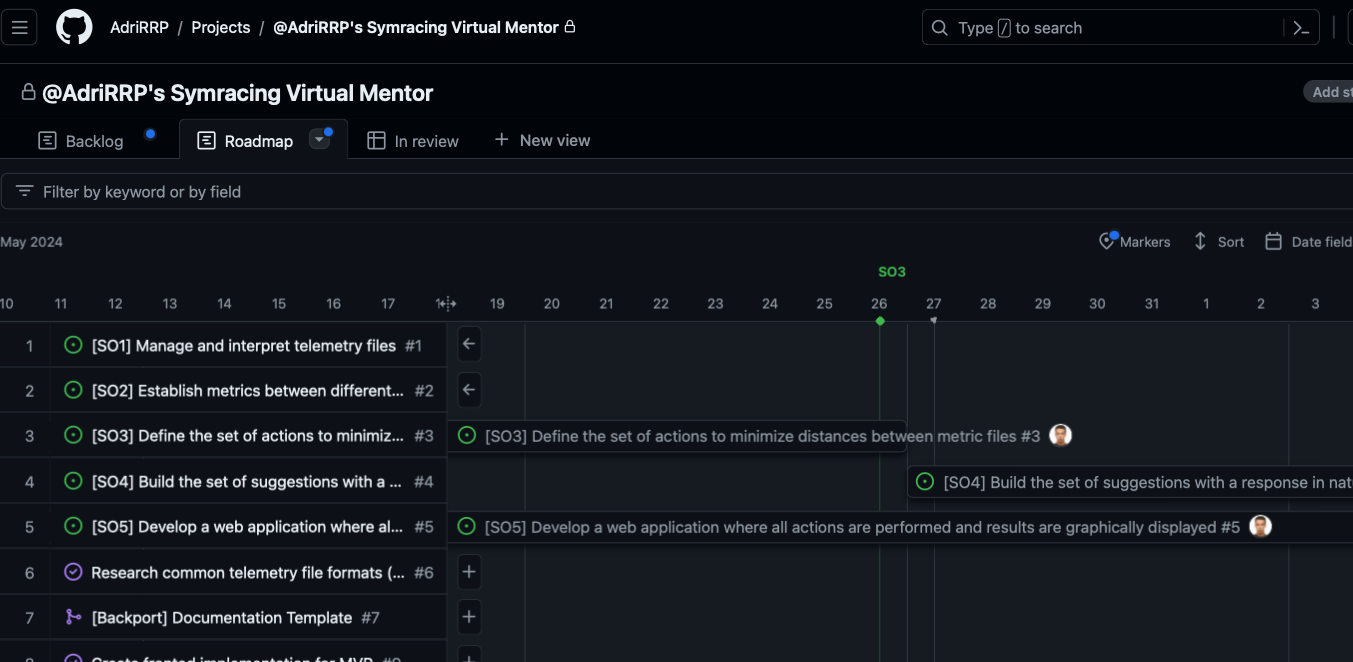
\includegraphics[width=0.8\linewidth]{./figs/herramientas/desarrollo/ghproject_roadmap.png}
	\caption[Captura de roadmap de GitHub Projects]{Captura de roadmap de GitHub Projects}
 \label{fig:ghp_milestones}
\end{figure}


El uso del tablero de tareas en GitHub Projects ha sido una herramienta fundamental en la gestión ágil de este proyecto, proporcionó una visualización clara y estructurada del flujo de trabajo además de facilitar la colaboración y el seguimiento del progreso. El tablero de GitHub Projects se organizó en cinco paneles distintos: ''milestones'' (hitos), ''backlog'' (lista de tareas pendientes), ''in progress'' (en curso), ''ready'' (listas para ser ejecutadas) y ''done'' (finalizadas) (\autoref{fig:ghp_board}).

\begin{figure}[H]
	\centering
	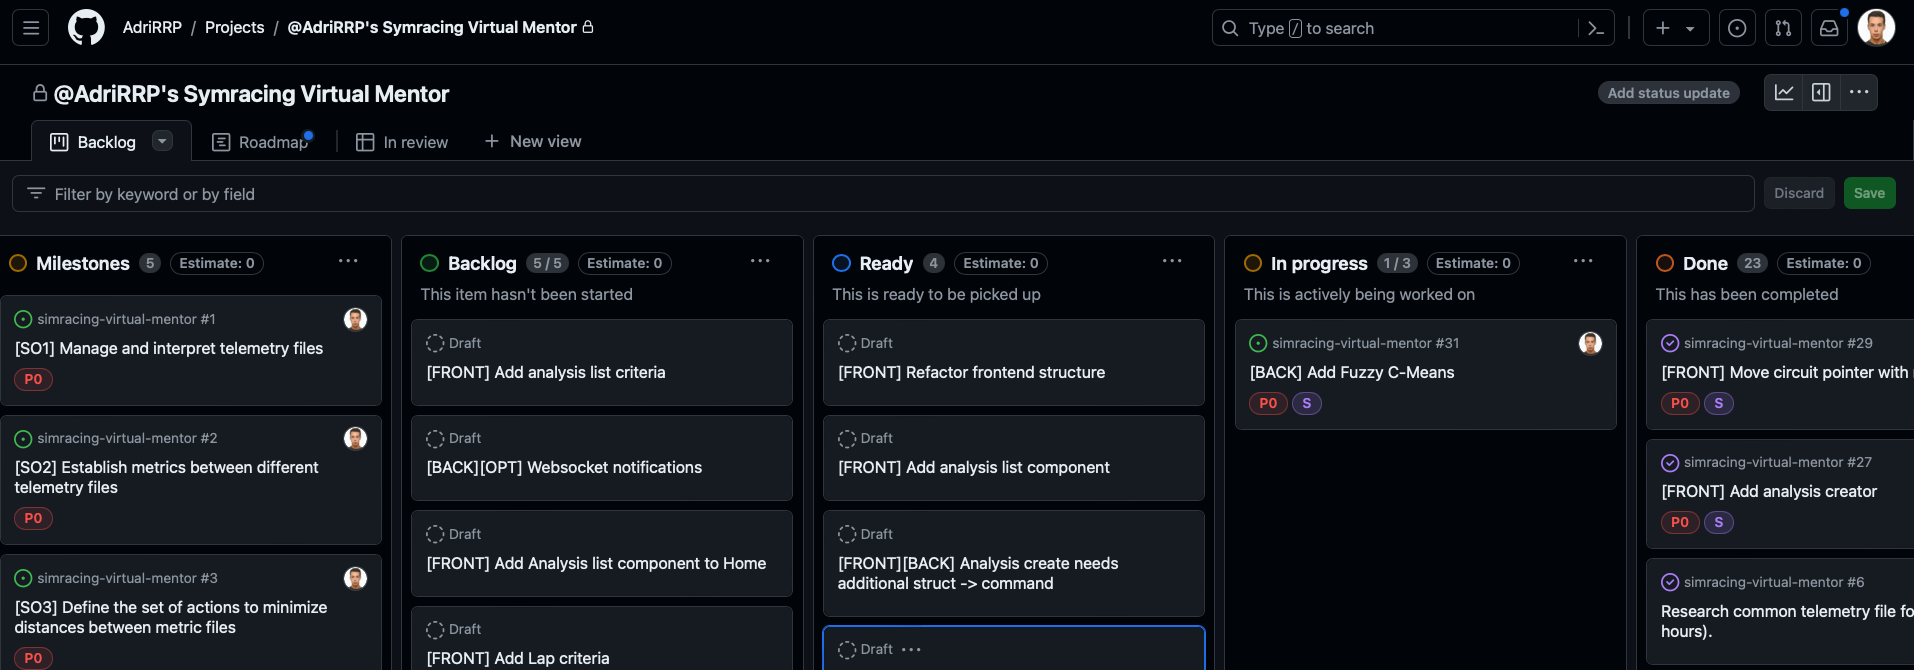
\includegraphics[width=0.9\linewidth]{./figs/herramientas/desarrollo/ghproject_board.png}
	\caption[Captura de tablero de GitHub Projects]{Captura de tablero de GitHub Projects}
    \label{fig:ghp_board}
\end{figure}

\begin{itemize}[noitemsep]
\item El panel \textbf{''milestones''} permitió a los miembros del equipo visualizar el progreso de los hitos de un vistazo, asegurando que los objetivos a largo plazo se  mantenían en el horizonte y se alineaban con las expectativas del cliente.
\item El panel \textbf{''backlog''} contenía todas las tareas necesarias para completar los hitos, proporcionando un depósito centralizado de trabajo pendiente que se gestionó y priorizó continuamente.
\item El panel \textbf{''ready''} indicaba qué tareas estaban listas para ser abordadas tras haber pasado por el proceso de refinamiento y priorización.
\item El panel \textbf{''in progress''} mostraba las tareas que estaban desarrollándose, permitiendo al equipo y a los interesados ver qué trabajo se estaba llevando a cabo en tiempo real.
\item El panel \textbf{''done''} contenía las tareas completadas, ofreciendo una visión clara de lo que ya se había logrado y ayudando a medir el progreso de los objetivos establecidos.\\
\end{itemize}

Desde GitHub Projects también se gestionaron las incidencias. Cada incidencia se daba de alta con un título y una descripción, además se le asignaba un estado inicial de borrador (draft). Durante las reuniones de planificación del sprint, en las que se revisaba el progreso y se establecían nuevos objetivos con el cliente, se examinaban estas incidencias o se creaban nuevas. Se les asignaba una prioridad (etiquetadas como P0, P1 o P2) para indicar su urgencia. Además, cada incidencia recibía una talla, un concepto similar a los puntos de esfuerzo de Scrum que cuantifica el esfuerzo requerido, utilizando una escala similar a los tamaños de ropa, que va desde XS hasta XL (\autoref{fig:ghp_issue}). Posteriormente, la incidencia se movía al backlog para que el programador pudiera asignársela.

\begin{figure}[H]
	\centering
	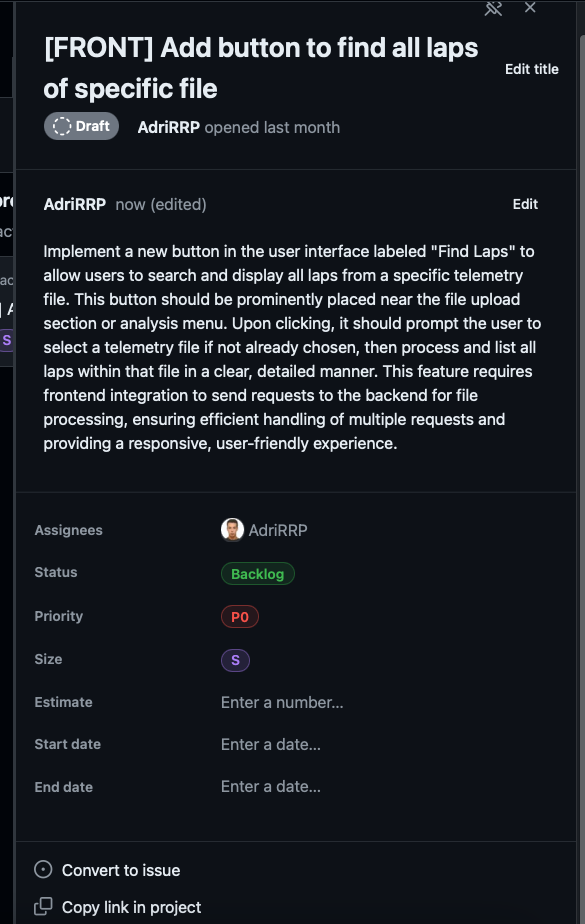
\includegraphics[width=0.30\linewidth]{./figs/herramientas/desarrollo/ghproject_issue.png}
	\caption[Captura de incidencia de GitHub Projects]{Captura de incidencia de GitHub Projects}
    \label{fig:ghp_issue}
\end{figure}

\subsection{Domain Driven Design \textit{(\ac{ddd}}) y Arquitectura Hexagonal}
La adopción de \ac{ddd} y la Arquitectura Hexagonal en este proyecto fue una decisión estratégica que permitió manejar la complejidad y asegurar la flexibilidad y escalabilidad del entrenador virtual de Simracing.

\begin{itemize}[noitemsep]
\item \textbf{Domain-Driven Design}: \ac{ddd} se centra en construir un modelo de dominio que refleje con precisión los conceptos y reglas del dominio específico del negocio. En este proyecto, se ha aplicado \ac{ddd} para estructurar las capas de dominio y aplicación de manera efectiva, asegurando que la lógica de negocio esté bien definida y separada de las preocupaciones técnicas. Esto permite una mejor alineación con los requisitos del cliente y facilita la colaboración entre desarrolladores y expertos en el dominio \cite{Evans2004}. La estructura de directorios del proyecto refleja esta separación, con módulos claramente definidos para diferentes partes del dominio, como \textit{ibt\_extractor, analysis, file y lap}.
\item \textbf{Arquitectura Hexagonal}: La Arquitectura Hexagonal, propuesta por Alistair Cockburn, busca desacoplar el núcleo de la aplicación de las interfaces externas (\autoref{fig:hex_arch}), permitiendo que el sistema sea más adaptable a cambios futuros y facilitando la integración con nuevas tecnologías \cite{Cockburn2005}. En este proyecto, la arquitectura hexagonal se ha implementado mediante la separación de los componentes de la aplicación en capas bien definidas, con directorios dedicados a infraestructura, aplicación, y dominio. Esto no sólo ha mejorado la mantenibilidad del código, sino que también ha permitido realizar pruebas más efectivas y gestionar la complejidad de manera más eficiente.
\end{itemize}

\begin{figure}[H]
	\centering
	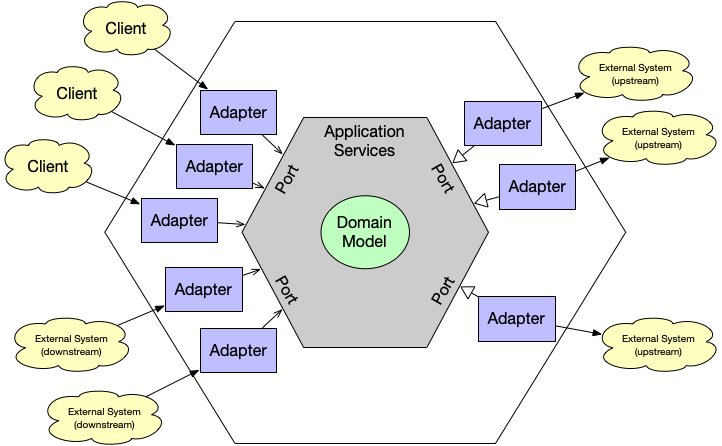
\includegraphics[width=0.5\linewidth]{./figs/herramientas/desarrollo/hexagonal.png}
	\caption[Esquema de Arquitectura Hexagonal]{Esquema de Arquitectura Hexagonal \cite{hexagonal_architecture}}
    \label{fig:hex_arch}
\end{figure}

La combinación de \ac{ddd} y la Arquitectura Hexagonal en este proyecto ha permitido desarrollar un sistema modular y escalable, con un backend robusto basado en principios de diseño estratégico y táctico. El uso de eventos y suscriptores en el backend, junto con la implementación de controladores y repositorios, ha asegurado que la lógica de negocio esté desacoplada de las interfaces técnicas, facilitando la evolución del sistema según las necesidades de los clientes.

\section{Recursos}
En esta sección se detallan los recursos que han sido necesarios para la realización del proyecto, clasificados en hardware, software y humanos, éstos últimos revisados en la sección \hyperref[sec:impl_xp]{metodología de desarrollo}. Además, se incluye una estimación del coste total del proyecto basada en estos recursos. Este análisis ha permitido una comprensión clara de las inversiones requeridas y de cómo se han distribuido los esfuerzos, así como las herramientas empleadas para el desarrollo del asistente virtual de Simracing.

\subsection{Recursos Hardware}
En esta sección se describen los recursos hardware utilizados durante  el desarrollo del proyecto. Este análisis incluye tanto los componentes principales del hardware como sus características relevantes.

\begin{itemize}
\item MacBook Pro M2 (Apple M2 Pro, 16GB RAM, 1TB SSD, monitor Liquid Retina XDR 14 pulgadas).
\item 2 Monitores Phillips Brilliance 241B (24 pulgadas, Full HD).
\item Ratón MSI Interceptor DS300 (7.200 DPI, ergonómico).
\item Teclado Razer Huntsman (mecánico, retroiluminado).
\item Estación de anclado StarTech DK30A2DHU (USB-C, dual HDMI).
\item Router TP-Link Archer AX50.
\end{itemize}

\begin{figure}[H]
	\centering
	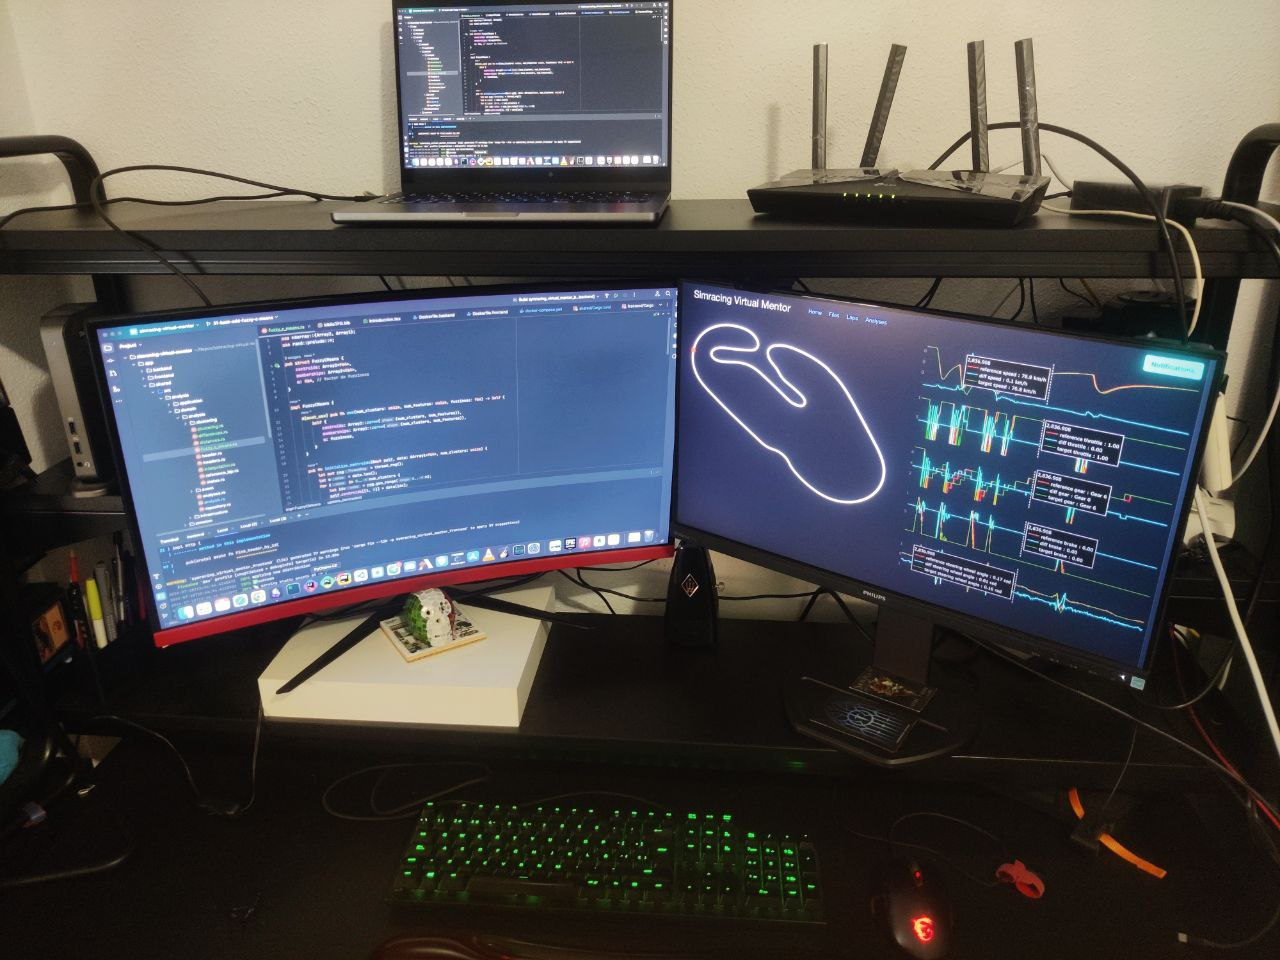
\includegraphics[width=0.70\linewidth]{./figs/herramientas/hardware/recursos_hardware.png}
	\caption[Recursos Hardware utilizados]{Recursos Hardware utilizados}
    \label{fig:recursos_hardware}
\end{figure}


\subsection{Recursos Software}
\subsubsection*{Sistemas Operativos}
\begin{itemize}
\item macOS Sonoma 14.5 (23F79) \cite{macos14_5_release_notes}
\end{itemize}

\subsubsection*{Lenguajes}
\begin{itemize}
\item Programación
    \begin{itemize}
    \item \textbf{Rust 1.79.0}: Lenguaje de programación que enfatiza seguridad, concurrencia y eficiencia, ideal para desarrollar aplicaciones de alto rendimiento sin comprometer la robustez \cite{rust_release_notes_1_79}.
    \end{itemize}
\item Scripting
    \begin{itemize}
    \item \textbf{JavaScript}: Lenguaje de programación interpretado que se utiliza para el desarrollo de aplicaciones web dinámicas y la manipulación del \ac{dom} \cite{mozilla_js}.
    \item \textbf{Dockerfile Syntax}: Lenguaje de configuración utilizado para definir entornos y aplicaciones Docker mediante instrucciones y comandos específicos en un archivo de texto estructurado \cite{dockerfile}.
    \item \textbf{Bash}: Lenguaje de scripting utilizado en sistemas Unix para automatización de tareas y gestión de comandos \cite{bash}.
    \end{itemize}
\item Marcado
    \begin{itemize}
    \item \textbf{\ac{html}}: Lenguaje de marcado  estándar para crear y estructurar páginas web \cite{html}.
    \item \textbf{\ac{json}}: Formato ligero de intercambio de datos fácil de leer y escribir \cite{json}.
    \item \textbf{\ac{yaml}}: Formato de serialización de datos legible por humanos que se utiliza principalmente para archivos de configuración \cite{yaml}.
    \item \textbf{\ac{toml}}: Lenguaje de marcado diseñado para la configuración, enfocándose en la simplicidad y legibilidad humana \cite{toml}.
    \end{itemize}
\item Estilo
    \begin{itemize}
    \item \textbf{\ac{css}}: Lenguaje de estilo usado para describir la presentación de un documento \ac{html} \cite{rust_release_notes_1_79}.
    \end{itemize}
\end{itemize}
\subsubsection*{Bases de Datos}
\begin{itemize}
\item \textbf{MongoDB 7.0} Base de datos NoSQL orientada a documentos \cite{mongodb}.
\item \textbf{MongoDB Compass 1.43.1}: interfaz gráfica para MongoDB que permite explorar, analizar y manipular los datos \cite{mongodb_compass}.
\end{itemize}

\subsubsection*{Librerías}
\begin{itemize}
\item Rust
    \begin{itemize}
    \item \textbf{async-trait 0.1.80}: Permite definir y utilizar traits asíncronos en Rust \cite{async_trait}.
    \item \textbf{axum 0.7.5}: Framework para construir aplicaciones web en Rust con soporte para Tokio \cite{axum}.
    \item \textbf{base64 0.22.1}: Librería para la codificación y decodificación de datos en Base64 \cite{base64}.
    \item \textbf{bson 2.11.0}: Implementación de BSON para Rust, utilizada para trabajar con MongoDB \cite{bson}.
    \item \textbf{chrono 0.4.38}: Librería para la manipulación y formateo de fechas y tiempos \cite{chrono}.
    \item \textbf{config 0.14.0}: Proporciona soporte para la configuración basada en archivos y entornos \cite{config}.
    \item \textbf{futures 0.3.30}: Librería para la programación asíncrona y manejo de futuros en Rust \cite{futures}.
    \item \textbf{futures-util 0.3.30}: Utilidades adicionales para trabajar con futuros en Rust \cite{futures_util}.
    \item \textbf{gloo 0.11.0}: Conjunto de utilidades para el desarrollo de aplicaciones web en Rust \cite{gloo}.
    \item \textbf{gloo-events 0.1}: Librería para trabajar con eventos en aplicaciones web \cite{gloo_events}.
    \item \textbf{gloo-net 0.5.0}: Librería para realizar solicitudes de red en aplicaciones web \cite{gloo_net}.
    \item \textbf{js-sys 0.3.69}: Enlaza cada \ac{api} del sistema JavaScript con Rust \cite{js_sys}.
    \item \textbf{log 0.4.21}: Proporciona una interfaz de registro de logs para Rust \cite{log}.
    \item \textbf{mime 0.3.17}: Librería para trabajar con tipos MIME \cite{mime}.
    \item \textbf{mockall 0.12.1}: Herramienta para crear mocks en Rust durante las pruebas \cite{mockall}.
    \item \textbf{mongodb 2.8.2}: Cliente oficial de MongoDB para Rust \cite{mongodb_crate}.
    \item \textbf{ndarray 0.15.6}: Librería para el manejo de arreglos multidimensionales en Rust \cite{ndarray}.
    \item \textbf{plotly 0.8.4}: Librería para crear gráficos interactivos en Rust \cite{plotly}.
    \item \textbf{rand 0.8.5}: Librería para la generación de números aleatorios \cite{rand}.
    \item \textbf{reqwest 0.12.4}: Cliente \ac{http} simple y eficaz para Rust \cite{reqwest}.
    \item \textbf{serde 1.0.203}: Librería de serialización y deserialización en Rust \cite{serde}.
    \item \textbf{serde-json 1.0.117}: Extensión de Serde para trabajar con JSON \cite{serde_json}.
    \item \textbf{serde-wasm-bindgen 0.6.5}: Librería para la serialización y deserialización con wasm-bindgen \cite{serde_wasm_bindgen}.
    \item \textbf{serde-yaml 0.9}: Extensión de Serde para trabajar con YAML \cite{serde_yaml}.
    \item \textbf{sha256 1.5.0}: Librería para calcular hashes SHA-256 \cite{sha256}.
    \item \textbf{thiserror 1.0.61}: Proporciona una manera ergonómica de definir errores \cite{thiserror}.
    \item \textbf{tokio 1.38.0}: Runtime asíncrono para Rust con soporte para I/O y timers \cite{tokio}.
    \item \textbf{tower-http 0.5.2}: Conjunto de utilidades y middleware para trabajar con servicios \ac{http} \cite{tower_http}.
    \item \textbf{tracing 0.1.40}: Librería para instrumentar aplicaciones Rust para el registro de logs estructurados \cite{tracing}.
    \item \textbf{tracing-subscriber 0.3.18}: Colección de suscriptores para manejar la salida de tracing \cite{tracing_subscriber}.
    \item \textbf{urlencoding 2.1.3}: Librería para la codificación y decodificación de URLs \cite{urlencoding}.
    \item \textbf{uuid 1.8.0}: Librería para la generación y manejo de \ac{uuid} \cite{uuid}.
    \item \textbf{wasm-bindgen 0.2.92}: Proporciona soporte para la interoperabilidad entre Rust y WebAssembly \cite{wasm_bindgen}.
    \item \textbf{wasm-bindgen-futures 0.4.42}: Extensión de wasm-bindgen para trabajar con futuros \cite{wasm_bindgen_futures}.
    \item \textbf{wasm-bindgen-file-reader 1.0.0}: Librería para la lectura de archivos en aplicaciones WebAssembly \cite{wasm_bindgen_file_reader}.
    \item \textbf{wasm-logger 0.2.0}: Implementación de un logger para aplicaciones WebAssembly \cite{wasm_logger}.
    \item \textbf{web-sys 0.3.69}: Enlaza las \ac{api}s del sistema Web con Rust \cite{web_sys}.
    \item \textbf{yew 0.21}: Framework para el desarrollo de aplicaciones web con WebAssembly \cite{yew}.
    \item \textbf{yew-hooks 0.3.2}: Conjunto de hooks para el framework Yew \cite{yew_hooks}.
    \item \textbf{yew-router 0.18.0}: Librería para el enrutamiento en aplicaciones Yew \cite{yew_router}.
    \end{itemize}
\item JavaScript
    \begin{itemize}
    \item \textbf{Plotly JS 2.33.0}: Librería de gráficos interactivos \cite{plotly_js}.
    \end{itemize}
\item \ac{css}
    \begin{itemize}
    \item \textbf{Bulma 1.0.0}: Framework \ac{css} moderno y adaptable. 
    \end{itemize}
\end{itemize}

\subsubsection*{Herramientas de construcción}
\begin{itemize}
\item \textbf{Cargo 1.79.0}: Gestor de paquetes Rust \cite{rust_cargo}.
\item \textbf{Trunk 0.20.2}: Herramienta para construir y desplegar aplicaciones Web basadas en WebAssembly para Rust \cite{trunk}.
\item \textbf{xx 1.4.0}: Herramienta de compilación cruzada y multi-plataforma \cite{xx}.
\end{itemize}

\subsubsection*{Herramientas de desarrollo}
\begin{itemize}
\item \textbf{RustRover 2024.1}: Entorno de desarrollo para Rust \cite{rust_rover}.
\item \textbf{Vim 9.0}: Editor de texto avanzado \cite{vim}.
\item \textbf{xxd 1.4.0}: Herramienta para visualizar datos en hexadecimal \cite{xxd}.
\item \textbf{Google Chrome 126.0.6478.127}: Navegador web desarrollado por Google \cite{chrome}.
\end{itemize}

\subsubsection*{Documentación}
\begin{itemize}
\item \textbf{\LaTeX}: Sistema de preparación de documentos que utiliza macros y formato TEX \cite{latex_project}.
\item \textbf{Overleaf}: Plataforma colaborativa para redacción científica en LaTeX \cite{overleaf}.
\item \textbf{ChatGPT 4o}: Modelo de lenguaje desarrollado por OpenAI utilizado para asistir en la redacción, estructuración y documentación del contenido de este proyecto \cite{chatgpt}.
\end{itemize}

\subsection{Coste}
En esta sección se realiza una estimación de los costes totales del proyecto, teniendo en cuenta los recursos hardware y humanos necesarios. El software utilizado es de carácter libre, por lo que no se incluye en la estimación de costes. A continuación se presentan los detalles y cálculos:
\begin{itemize}
    \item \textbf{Costes de recursos humanos:}
    \begin{itemize}
    \item Desarrollador Rust (nivel medio): 200 horas.
    \item Gerentes (clientes/directores del trabajo): 20 horas cada uno.
    \item Consultor experto en Simracing: 8 horas.
    \end{itemize}

    \item Según los datos del mercado laboral en España \cite{randstad,glassdoor,kiwiremoto}:
    \begin{itemize}
    \item Salario medio de un desarrollador Rust nivel medio: 25 €/hora.
    \item Salario medio de un gerente: 35 €/hora.
    \item Salario medio de un consultor: 45 €/hora.
    \end{itemize}

    \item \textbf{Costes de recursos hardware:}
    \begin{itemize}
    \item MacBook Pro M2 Pro de 14 pulgadas: 2.400 €.
    \item 2 Monitores Phillips Brilliance 241B: 400 € (200 € cada uno).
    \item Ratón MSI Interceptor DS300: 50 €.
    \item Teclado Razer Huntsman: 150 €.
    \item Estación de anclado StarTech DK30A2DHU: 200 €.
    \item Router TP-Link Archer AX50: 150 €.
    \end{itemize}

    \item \textbf{Cálculo de costes:}
    \begin{itemize}
    \item Coste del desarrollador: 200 horas * 25 €/hora = 5.000 €.
    \item Coste de los gerentes: 2 * 20 horas * 35 €/hora = 1.400 €.
    \item Coste del consultor: 8 horas * 45 €/hora = 360 €.
    \item Coste total del hardware: 2.400 € + 400 € + 50 € + 150 € + 200 € + 150 € = 3.350 €.
    \end{itemize}
\end{itemize}

\begin{table}[H]
\centering
\begin{tabular}{|l|c|}
\hline
\textbf{Recurso} & \textbf{Coste (€)} \\ \hline
Desarrollador (200 horas a 25 €/hora) & 5.000 \\ \hline
Gerentes (2 personas, 20 horas cada una a 35 €/hora) & 1.400 \\ \hline
Consultor (8 horas a 45 €/hora) & 360 \\ \hline
MacBook Pro M2 Pro de 14 pulgadas & 2.400 \\ \hline
2 Monitores Phillips Brilliance 241B & 400 \\ \hline
Ratón MSI Interceptor DS300 & 50 \\ \hline
Teclado Razer Huntsman & 150 \\ \hline
Estación de anclado StarTech DK30A2DHU & 200 \\ \hline
Router TP-Link Archer AX50 & 150 \\ \hline
Electricidad (uso proporcional: 20\% de 6 meses a 50 €/mes) & 60 \\ \hline
Internet (uso proporcional: 50\% de 6 meses a 30 €/mes) & 90 \\ \hline
\textbf{Total} & \textbf{10.260} \\ \hline
\end{tabular}
\caption{Coste total del proyecto desglosado por recursos}
\label{tab:costes_proyecto}
\end{table}

\section{Aseguramiento de la Calidad}
El aseguramiento de la calidad en este proyecto fue gestionado de manera integral utilizando varias estrategias y herramientas clave. A continuación se describe cómo se aplicaron estas medidas.

\subsection{Pruebas}
Rust ofrece un robusto sistema de testing integrado que se utilizó para realizar las pruebas del entrenador virtual de Simracing.
Se utilizó el enfoque de \ac{ddd} para estructurar el proyecto de manera que la lógica de negocio estuviera bien definida y aislada. Esto facilitó la creación de \textbf{pruebas unitarias} para el dominio de la aplicación.
Las \textbf{pruebas de integración} verificaron la coherencia y el correcto funcionamiento de los diferentes servicios (casos de uso/historias de usuario) sin necesidad de disponer de la infraestructura (repositorios y servicios externos) y por tanto sin acoplarse a ella. Esto fue posible gracias a \ac{ddd} y la separación entre las capas de aplicación e infraestructura.


\subsection{Análisis y Formato de Código}
Para mantener un formato de código estándar y mejorar la calidad del mismo, se utilizaron las herramientas \textbf{Cargo fmt} y \textbf{Clippy}. Cargo fmt aseguró que todo el código siguiera las convenciones de estilo de Rust, mejorando la legibilidad y facilitando la colaboración entre desarrolladores. Clippy se utilizó para realizar análisis estáticos del código, identificando posibles errores, malas prácticas y sugiriendo mejoras.


\subsection{Flujo de \ac{cicd} con GitHub Actions}
Se estableció un flujo de integración y entrega continua \ac{cicd} utilizando GitHub Actions \cite{github_actions}. Este flujo automatizado aseguraba que todos las pruebas se ejecutaran antes de integrar cambios en la rama principal (main). El proceso de \ac{cicd} incluía controles de calidad que utilizaban Codecov \cite{codecov} para medir la cobertura de los tests y garantizar que se mantenían altos estándares de calidad.

Los tres archivos clave en la carpeta `.github/workflows` fueron:
\begin{itemize}
    \item \textbf{clippy.yaml}: Configuración para ejecutar clippy y asegurar que el código seguía las mejores prácticas.
    \item \textbf{coverage.yaml}: Configuración para medir la cobertura de los tests con Codecov.
    \item \textbf{tests.yaml}: Configuración para ejecutar todos los tests unitarios e integrados del proyecto.
\end{itemize}

Estas prácticas permitieron identificar y corregir errores de manera temprana y aseguraron que el código cumpliera consistentemente con los estándares de calidad definidos. El uso de estas herramientas y metodologías no sólo mejoró la calidad del software, sino que también facilitó un desarrollo más ágil y eficiente.

\section{Riesgos}
Al inicio del proyecto de desarrollo del entrenador virtual para Simracing, se identificaron y evaluaron varios riesgos potenciales que podrían afectar el éxito del mismo. Estos riesgos se abordaron con un enfoque sistemático para mitigar su impacto y garantizar un desarrollo fluido.

\begin{itemize}
    \item Uno de los riesgos principales identificados fue la \textbf{complejidad técnica del proyecto}. La implementación de \ac{ddd} y la Arquitectura hexagonal implicaba un nivel elevado de abstracción y modularidad que requería una comprensión profunda de estos conceptos por parte del desarrollador. Esto se mitigó mediante el estudio y la aplicación gradual de estas metodologías, así como con la consultoría especializada de un experto en Simracing.
    \item Otro riesgo significativo fue la \textbf{integración de tecnologías y herramientas diversas}. La utilización de Rust como lenguaje principal, junto con MongoDB para la gestión de datos, y herramientas como GitHub Actions para \ac{cicd}, requería una integración cuidadosa y coordinada. Para mitigar este riesgo, se definieron claramente las responsabilidades de cada componente del sistema y se implementaron pruebas unitarias e integradas para asegurar la correcta interoperabilidad.
    \item Además, la \textbf{gestión de la calidad del código} se identificó como un riesgo crucial. La utilización de Clippy y Cargo fmt fue esencial para mantener un estándar de codificación elevado y consistente. Sin embargo, se reconoció que la configuración de estas herramientas podría ser desafiante y consumir tiempo. Este riesgo se manejó configurando Clippy con sus vertientes más restrictivas desde el inicio y asegurando que el desarrollador se familiarizara con su uso.
    \item Finalmente, el riesgo asociado al \textbf{despliegue y mantenimiento del sistema} se abordó mediante la implementación de un flujo de \ac{cicd} robusto utilizando GitHub Actions y Codecov. Este enfoque permitió una integración continua y un despliegue controlado, minimizando los errores y asegurando una cobertura de pruebas adecuada antes de cualquier fusión en la rama principal del proyecto.
\end{itemize}

En resumen, la identificación y gestión proactiva de estos riesgos fue fundamental para el éxito del proyecto, permitiendo abordar desafíos técnicos complejos y asegurar un alto nivel de calidad en el desarrollo del entrenador virtual para Simracing.